% --
% adversarial

\section{Adversarial Training Theory}\label{sec:nn_adv}
Working with adversarial Neural Networks is quite interesting, as two separate Networks are challenge themselves against each other to improve their performance.
The paper from Goodfellow et. al. \cite{goodfellow2014} describes a game between two Neural Networks (players), where one player has the role of creating fakes and the other must determine if it is real or fake.
The Network who creates fakes is called Generator (G) and the other Network who has to decide about fake or not is called Discriminator (D).
The Generators goal is to create fakes that look like reals, so that D makes mistakes and classifies a fake as a real.
On the other hand the Discriminator must also constantly improving itself, so that fakes from G can be detected and sorted out from the reals.

This approach works remarkably well to create a generative network able to produce fakes that are astonishing similar to real ones.
In the mentioned paper, this was applied to images and not for audio data.
But if the audio waveform is presented as spectogram or mfcc with fixed frame size, it can be seen as an image, where one dimension is time and the other frequency.

So far a generative network does only produce fake images and a discriminative network can only output a one dimensional (probability) output, to decide if it is fake or not.

The idea now is not to use either of these networks, but to use transfer learning in the sense to reuse the convolutional layers both networks achieved during their game (training).
The weights of those convolutional layers are then transfered to another network with classification purpose on multiple labels.

\subsection{Questions that arise}
There are several questions that arise regarding Adversarial Training:
\begin{enumerate}[label={Q.\textgoth{A}.\arabic*)}, leftmargin=1.4cm]
  \item Does the Network Architecture of G and D have to be the same but transposed?
  \item Does the value space of in and outputs, for D and G respectively, have to be limited e.g. [0, 1] done by e.g. frame normalization, or sigmoid output?
  \item What loss function works well for training?
  \item How long should be trained?
  \item When transfering weights to another network, should the weights from G or D be transfered?
  \item Does the classification network has to adapt the parameters from the transfered weights?
  \item Whats the benefit of all this?
\end{enumerate}

To illustrate the idea an example is shown of the labels L5 (left, right, up, down, go).

The convolutional layer weights from the adversarial training of the individual labels, 
can be stacked together an used to initialize another network.
An example of this method is shown in \rfig{nn_adv_example}, where the initialization pattern changes to more elaborate structures and patterns to form good classification outputs. 
However the Basic Pattern from the adversarial training stays the same, which is a good sign, because then the network is accepting those trained weights and adapts them.

\begin{figure}[!ht]
  \centering
    \subfigure[c1 trained]{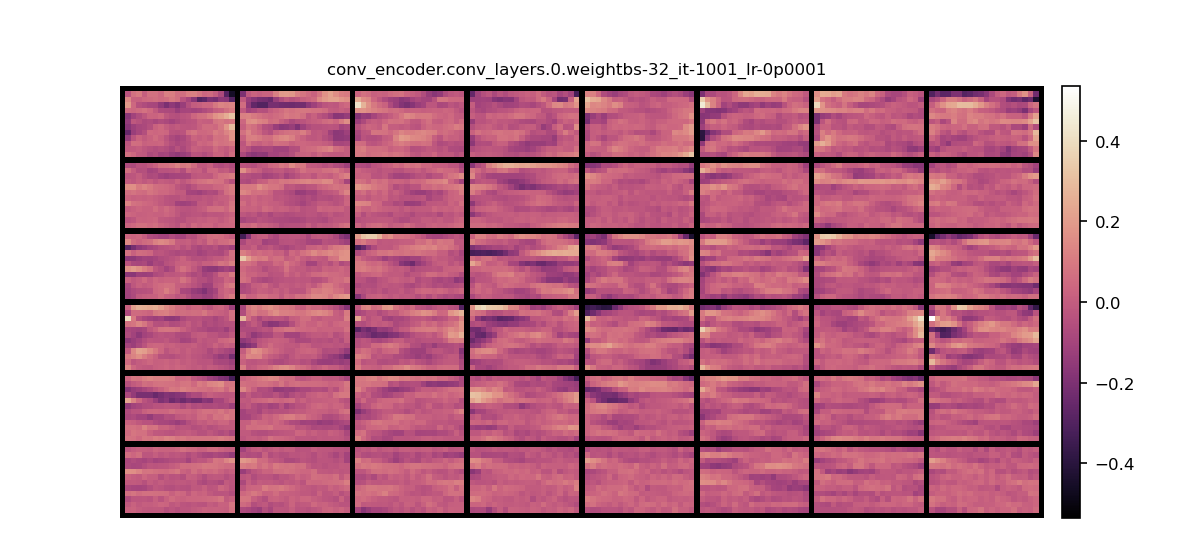
\includegraphics[width=0.45\textwidth]{./4_nn/figs/nn_adv_example_c0}}
    \subfigure[c1 init]{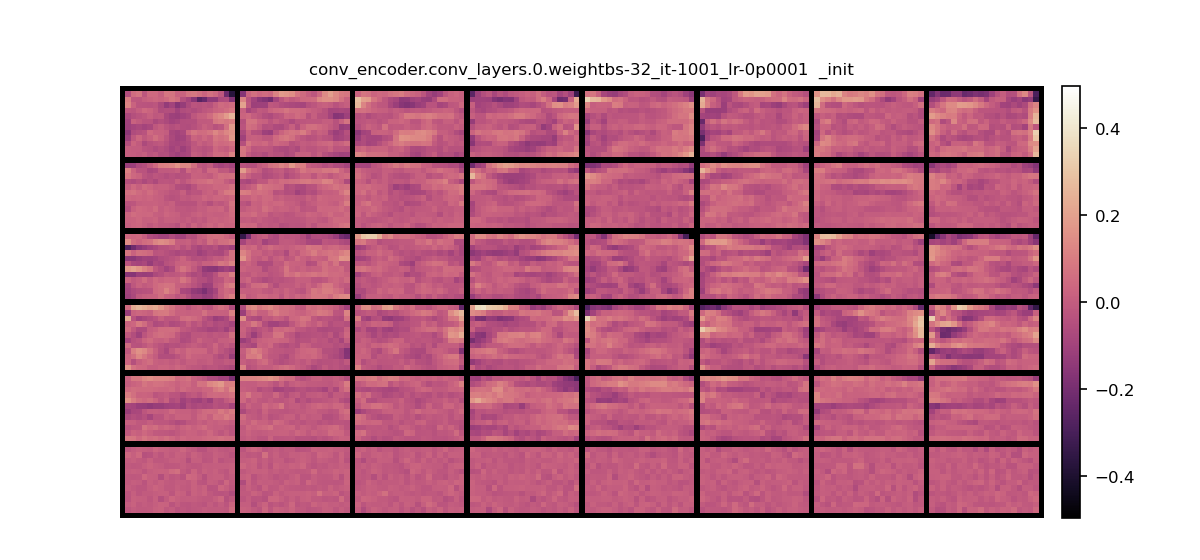
\includegraphics[width=0.45\textwidth]{./4_nn/figs/nn_adv_example_c0_init}}
    \subfigure[c2 trained]{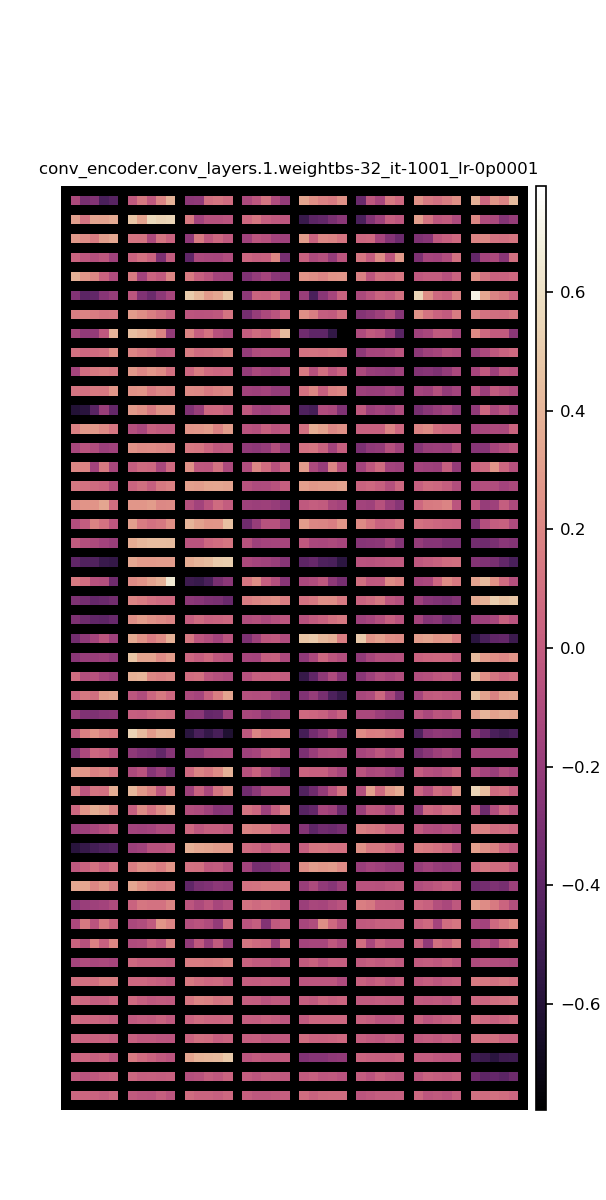
\includegraphics[height=0.45\textwidth]{./4_nn/figs/nn_adv_example_c1}}
    \quad
    \subfigure[c2 init]{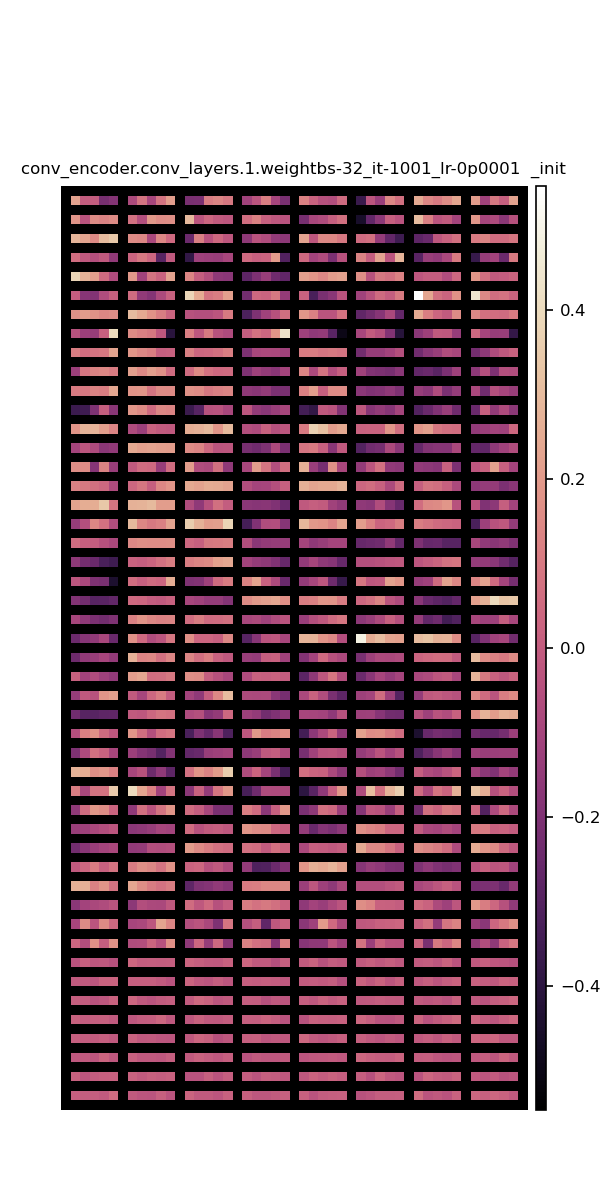
\includegraphics[height=0.45\textwidth]{./4_nn/figs/nn_adv_example_c1_init}}
  \caption{Adversarial Training Example: Convolutional layers pretrained with adversarial training on each label separately.}
  \label{fig:nn_adv_example}
\end{figure}
\FloatBarrier
\noindent

For this example in adversarial training, 8 feature maps of the first layer were used for each label, also they belong to the Generator Network G or decoder (dec). In Convolutional Networks, each previous layers feature map creates a new set of feature maps in the next layer.
An example of this label training is shown in \rfig{nn_adv_example_label} with feature maps [(1, 8), (8, 8)] of the convolutional layers

\begin{figure}[!ht]
  \centering
    \subfigure[\enquote{left} c1 from D]{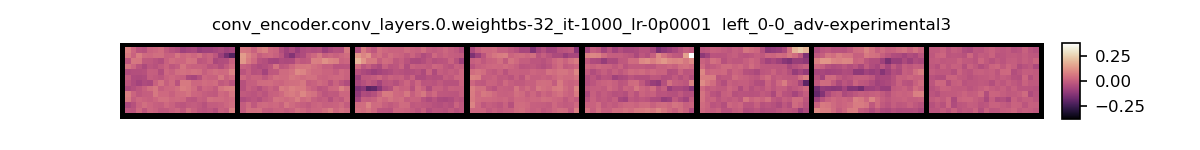
\includegraphics[width=0.45\textwidth]{./4_nn/figs/nn_adv_example_label_left_c0_enc}}
    \subfigure[\enquote{left} c1 from G]{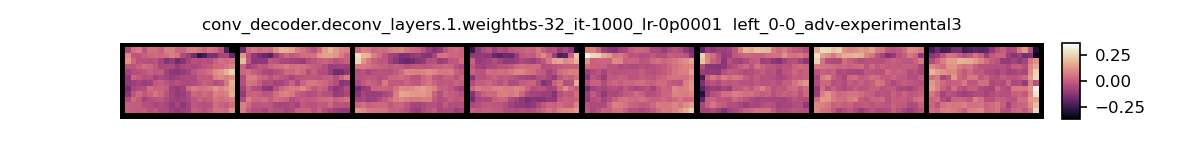
\includegraphics[width=0.45\textwidth]{./4_nn/figs/nn_adv_example_label_left_c0_dec}}
    \subfigure[\enquote{left} c2 from D]{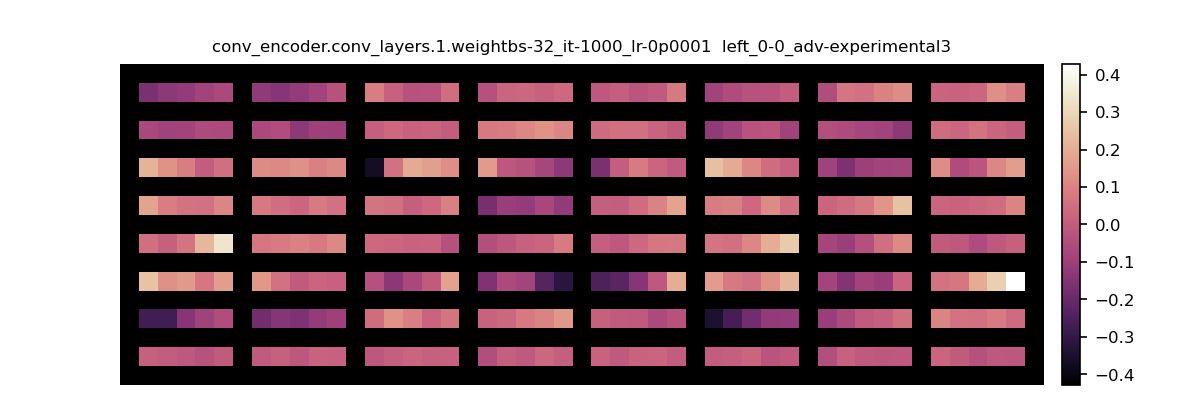
\includegraphics[width=0.3\textwidth]{./4_nn/figs/nn_adv_example_label_left_c1_enc}}
    \subfigure[\enquote{left} c2 from G]{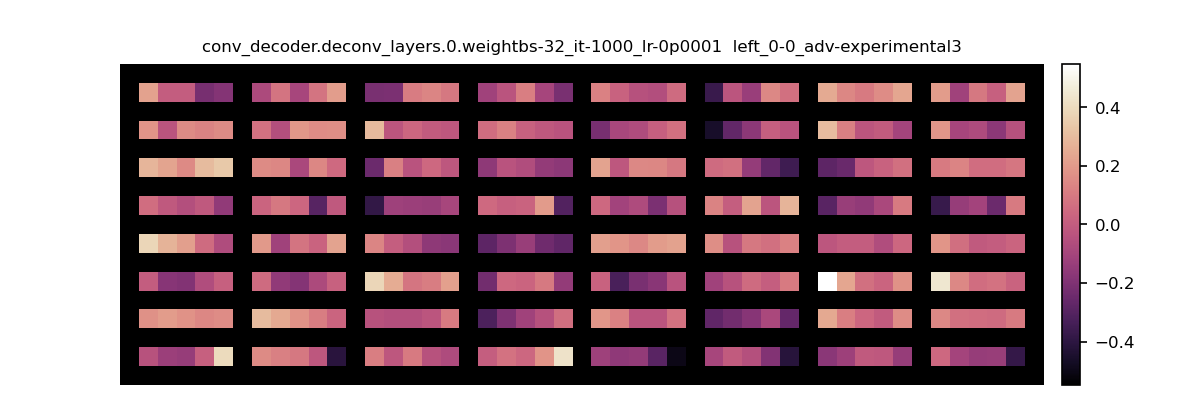
\includegraphics[width=0.3\textwidth]{./4_nn/figs/nn_adv_example_label_left_c1_dec}}
  \caption{Adversarial Training example of Generator (G) and Discriminator (D) of label \enquote{left} captured with 8 feature maps of the first convolutional layer.}
  \label{fig:nn_adv_example_label}
\end{figure}
\FloatBarrier
\noindent

Those trained weights from each label can then simply be put into the feature maps of a classification network.
This is shown in \rfig{nn_adv_example} where c1 from G and c2 from G in \rfig{nn_adv_example_label} were transfered to the first row(s).
When doing the transferring of feature maps, it is important that the layers are not mixed up so that the trained connections are still correct.
Also of course the weights of the feature maps must have the same dimension, so that transferring is possible.


\subsection{Observing the Generators output}
While the output of the Discriminator is rather uninteresting (one-dimensional probability value), the output of the Generator is a good indicator of how well the training between D and G has gone.
Optimally the output of the Generator look like real data samples.
An example of a trained Generator Network with fake outputs compared to real ones is shown in \rfig{nn_adv_gen}.

\begin{figure}[!ht]
  \centering
    \subfigure[\enquote{left} real examples]{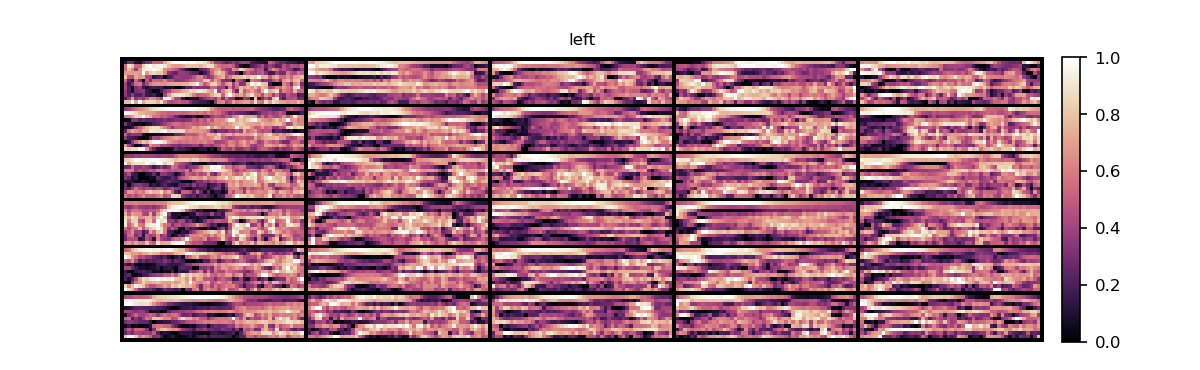
\includegraphics[width=0.45\textwidth]{./4_nn/figs/nn_adv_gen_left_real}}
    \subfigure[\enquote{left} fakes from G]{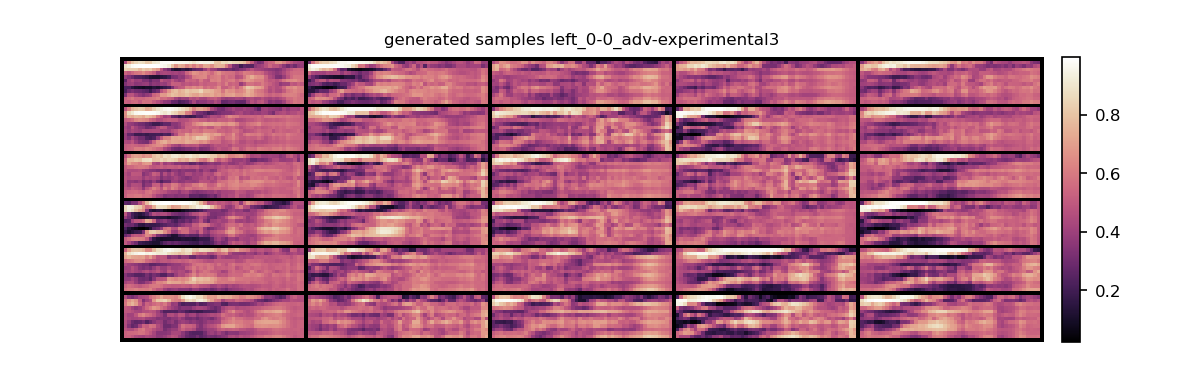
\includegraphics[width=0.45\textwidth]{./4_nn/figs/nn_adv_gen_left_fake}}
  \caption{Real samples of \enquote{left} from the Speech Commands dataset compared to fake samples from a trained Generator Network.}
  \label{fig:nn_adv_gen}
\end{figure}
\FloatBarrier
\noindent

If the fake example of the Generator Network do not look similar to real ones, then something might have gone wrong in the training between the Generator and Discriminator Network.
Further it can be evaluated if a certain network architecture is able to produce a label in a sufficient representation, therefore this method might be a good start in finding a suitable network architecture for the problem to be solved.



